
\chapter{Direct Correlation Function of Water\label{chpt:dcf-water}}

The bulk \acs{DCF}, which is an input for \acs{MDFT} and does not
depend on the solute, can be extracted from numerical simulations.
In this thesis, the SPC/E water is used as a solvent. Two sources of
bulk \acs{DCF} are used: 
\begin{enumerate}
\item The \acs{DCF} at dipolar order ($\hat{c}_{S}^{000}$, $\hat{c}_{\Delta}^{110}$,
$\hat{c}_{D}^{112}$) by Zhao \textit{et al.} \citep{zhao_accurate_2013}
using \acs{MD};
\item The complete \acs{DCF} up to a given order, for instance $n_{\max}=5$,
by Puibasset \textit{et al.} \citep{puibasset_bridge_2012} using
\acs{MC}.
\end{enumerate}

\section{Dipole DCF from molecular dynamics simulation}

The \acs{DCF} produced by Zhao \textit{et al.}, namely the dipole
\acs{DCF}, contains three primary rotational invariant projections
that correspond to $n_{\max}=1$. They are calculated with the
angular dependent \acs{PCF} in intermolecular frame, $h(r,\cos\theta_{1},\cos\theta_{2},\psi_{1},\psi_{2},\phi_{12})$,
which is directly extracted from \acs{MD} simulation. 

As the primary projections do not depend on the $\psi$ angles, the
intermolecular frame \acs{DCF} can be simplified as:
\begin{equation}
h(r,\boldsymbol{\omega}_{1},\boldsymbol{\omega}_{2})\equiv h(r,\cos\theta_{1},\cos\theta_{2},\phi_{12})=\left\langle h(r,\cos\theta_{1},\cos\theta_{2},\psi_{1},\psi_{2},\phi_{12})\right\rangle _{\psi_{1},\psi_{2}}\label{eq:h-linear}
\end{equation}
and in $k$-space:
\begin{equation}
h(k,\mathbf{\Omega}_{1},\mathbf{\Omega}_{2})=\int\mathrm{d}r\mathrm{d}\cos\theta_{r}\mathrm{d}\phi_{r}e^{ikr\cos\theta_{r}}h(r,\boldsymbol{\omega}_{1},\boldsymbol{\omega}_{2})
\end{equation}
where $\theta_{r}$ and $\phi_{r}$ are the orientations in spherical
coordinates for $\mathbf{r}$ and $\mathbf{\Omega}$ is in laboratory
coordinate system.

The correlation functions are then expanded on and projected onto a basis
of rotational invariants:
\begin{equation}
h^{nml}(k)=f^{nml}\left\langle h(k,\mathbf{\Omega}_{1},\mathbf{\Omega}_{2})\Phi^{nml}\right\rangle _{\mathbf{\Omega}_{1},\mathbf{\Omega}_{2}}
\end{equation}
with
\begin{align}
\Phi^{000} & =1\nonumber \\
\Phi^{110} & =\mathbf{\Omega}_{1}\cdot\mathbf{\Omega}_{2}\\
\Phi^{112} & =3(\hat{\mathbf{k}}\cdot\mathbf{\Omega}_{1})(\hat{\mathbf{k}}\cdot\mathbf{\Omega}_{2})-\mathbf{\Omega}_{1}\cdot\mathbf{\Omega}_{2}\nonumber 
\end{align}
and $f^{000}=1$, $f^{110}=3$, $f^{112}=3/2$, according to the convention
of Wertheim and Hansen.

To obtain the \acs{DCF}, the \acs{OZ} equation must be solved. It
is shown that the isotropic ($n_{\max}=0$) and dipolar ($n_{\max}=1$)
components are decoupled:
\begin{equation}
\hat{c}^{000}(k)=\frac{\hat{h}^{000}(k)}{1+n_{0}\hat{h}^{000}(k)}
\end{equation}
\begin{equation}
\hat{c}_{+}(k)=\frac{\hat{h}_{+}(k)}{1+\frac{2}{3}n_{0}\hat{h}_{+}(k)}
\end{equation}
\begin{equation}
\hat{c}_{-}(k)=\frac{\hat{h}_{-}(k)}{1-\frac{1}{3}n_{0}\hat{h}_{-}(k)}
\end{equation}
where
\begin{equation}
\hat{h}_{+}(k)=\hat{h}^{112}(k)+\frac{1}{2}\hat{h}^{110}(k)
\end{equation}
\begin{equation}
\hat{h}_{-}(k)=\hat{h}^{112}(k)-\hat{h}^{110}(k)
\end{equation}
and idem. for $\hat{c}$.

\section{DCF projections from bulk Monte Carlo simulation}

The complete \acs{DCF} up to $n_{\max}=5$, which is the default
\acs{DCF} used in this thesis, is calculated from the $g_{\mu\nu}^{mnl}(r)$
accumulated from \acs{MC} simulation \citep{puibasset_bridge_2012}
by resolving the inverted \acs{MOZ} equation
\begin{equation}
\ln y_{\alpha}(r)=\left\langle \ln\left[\sum_{\alpha'=1}^{\alpha_{\max}}g_{\alpha'}(r)\Phi_{\alpha'}(\tilde{\Omega})\right]\Phi_{\alpha}^{*}(\tilde{\Omega})\right\rangle +\beta v_{\alpha}(r)\label{eq:dcf-inverse-oz}
\end{equation}
with the closure
\begin{equation}
g_{\alpha}(r)=\begin{cases}
g_{\alpha}^{\mathrm{MC}}(r), & r\leq r_{\max}^{\mathrm{MC}}\\
\left\langle \exp\left[-\beta v(r,\tilde{\Omega})+\sum_{\alpha'}\gamma_{\alpha'}(r)\Phi_{\alpha'}(\tilde{\Omega})\right]\Phi_{\alpha}^{*}(\tilde{\Omega})\right\rangle , & r>r_{\max}^{\mathrm{MC}}
\end{cases}\label{eq:dcf-closure}
\end{equation}
where $\ln y=\gamma+b$ is the cavity function ($b$ the bridge function),
$\alpha$ the projection number, and $r_{\max}^{\mathrm{MC}}$ is
the maximum radius of the \acs{MC} simulation. Beyond $r_{\max}^{\mathrm{MC}}$,
$g$ can be obtained by the usual \acs{HNC} closure, and it is shown
that the projections are continuous at $r_{\max}^{\mathrm{MC}}$,
which means \acs{HNC} closure is enough to cope with long range correlation
functions. Note that the $\alpha_{\max}$'s for different $n_{\max}$'s
lead to slightly different \acs{DCF} results according to eq. (\ref{eq:dcf-inverse-oz},\ref{eq:dcf-closure}). 

The \acs{DCF} in $k$-space is obtained by Hankel transform.

The convention of rotational invariants adapts those of Blum, which
gives, for example, for $n_{\max}=1$:
\begin{align}
\Phi^{000} & =1\nonumber \\
\Phi^{011} & =i\mathbf{k}\cdot\mathbf{\Omega}_{1}\nonumber \\
\Phi^{101} & =i\mathbf{k}\cdot\mathbf{\Omega}_{2}\nonumber \\
\Phi^{110} & =-\sqrt{3}\mathbf{\Omega}_{1}\cdot\mathbf{\Omega}_{2}\\
\Phi^{112} & =\sqrt{\frac{3}{10}}\left[3\mathbf{(\mathbf{k}\cdot\mathbf{\Omega}_{1})(\mathbf{k}\cdot\mathbf{\Omega}_{2})-\Omega}_{1}\cdot\mathbf{\Omega}_{2}\right]\nonumber 
\end{align}


\section{Comparison between DCFs\label{subsec:Comparison-with-non-coupling}}

The comparison between the primary projections of the \acs{DCF}s
is given in figure \ref{fig:Comparison-dcf-ref}.

\begin{figure}[H]
\begin{centering}
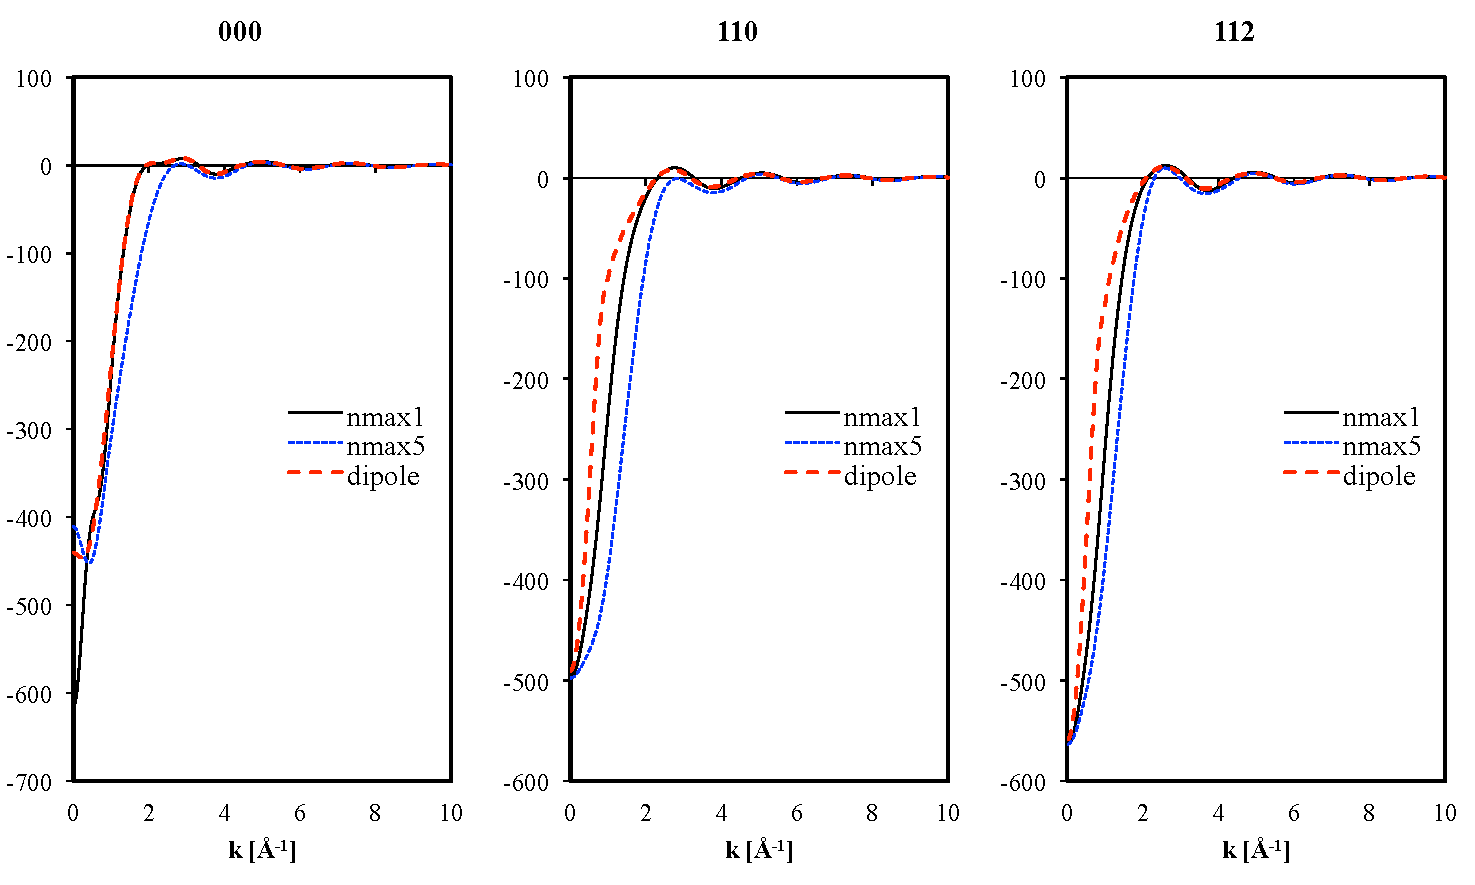
\includegraphics[width=1\columnwidth]{_figure/results/dcf}
\par\end{centering}
\caption[Comparison between \acs{DCF} projections]{Comparison between the \acs{DCF} projections of $n_{\max}=1$ (dipole)
from ref \citep{zhao_accurate_2013} and $n_{\max}=1,5$ from ref
\citep{puibasset_bridge_2012} (in convention of Wertheim and Hansen)\label{fig:Comparison-dcf-ref}}
\end{figure}

